\documentclass{beamer}
\usepackage{fancybox}
\usepackage{tikz}
\usetikzlibrary{arrows.meta,
                chains,
                positioning, 
                shadows.blur, shapes.arrows}
              
\usetheme{Madrid}

\title{Neuro-symbolic AI}
\author{Robert Hoehndorf}
\date{\today}

\begin{document}

\frame{\titlepage}

\begin{frame}
\frametitle{Overview}
\begin{itemize}
\item AI:
  \begin{itemize}
  \item Statistical
  \item Neural
  \item Symbolic
  \end{itemize}
\end{itemize}
\end{frame}

\begin{frame}
  \frametitle{Outline}
  \begin{itemize}
  \item Introduction
  \item Knowledge graphs, Question/Query answering
  \item Logic Programming
    \begin{itemize}
    \item ProbLog, ASP
    \item ILP
    \end{itemize}
  \item Markov Logic
  \item Fuzzy Logic and Logic Tensor Networks
  \item Geometric and algebraic methods, model theory
  \end{itemize}
\end{frame}

\begin{frame}
  \frametitle{Format and Evaluation}
  \begin{itemize}
  \item seminar-style course
    \begin{itemize}
    \item reading 2-3 research papers per week
    \item presentation (20\%) and discussion (20\%)
    \end{itemize}
  \item research project (60\%)
    \begin{itemize}
    \item start within the first 3 weeks
    \item individual project
    \item frequent project presentations/updates
    \item research paper
    \end{itemize}
  \end{itemize}
\end{frame}

\begin{frame}
  \frametitle{Research project}
  \begin{itemize}
  \item must combine neural/statistical and symbolic methods
  \item focus on either novel method or application
  \item aim at end of the course: research paper
    \begin{itemize}
    \item may be submitted to conference or journal
    \end{itemize}
  \end{itemize}
\end{frame}

\begin{frame}
  \frametitle{What is a viable research question?}
  \begin{itemize}
  \item qualitative (proof) vs quantitative (experiment)
  \item usually: improve method $X$ to address limitation $Y$
    \begin{itemize}
    \item $X$ --- existing method to solve some problem
    \item $Y$ --- how to find?
      \begin{itemize}
      \item analysis (primary research!)
      \item theoretical argument
      \item literature (check Discussion for limitations)
      \end{itemize}
    \end{itemize}
  \item or: develop method $X$ to overcome limitation $Y$ in methods
    addressing problem $Z$
  \end{itemize}
\end{frame}

\begin{frame}
  \frametitle{Examples}
  \begin{itemize}
  \item Can we develop an algorithm with $O(n \cdot \log{n})$ runtime
    that sorts a list of integers accurately in descending order?
    \pause
  \item Can graph neural networks improve reasoning over first order
    theories?
    \pause
    \begin{itemize}
    \item That is not a good research question on its own!
    \item How are current methods limited?
    \item How could GNNs overcome this limitation?
    \end{itemize}
  \end{itemize}
\end{frame}

\begin{frame}
  \frametitle{Answering the question}
  \begin{itemize}
  \item baseline
    \begin{itemize}
    \item how does method $X'$ solve problem $P$ now?
    \item quantify, and justify: which measure is appropriate? which
      test case / dataset is appropriate?
    \item are there different {\bf types} of methods to solve $P$? Did
      you include a representative for each?
    \item Why did you include method $X'$ over $X''$?
    \end{itemize}
    \pause
  \item workflow $W$: build a skeleton method to solve problem $P$
    \begin{itemize}
    \item can you reuse existing code? Check Github...
    \item you need to get from input (your dataset) to output (a
      number --- quantify!)
    \end{itemize}
    \pause
  \item actual methods research
    \begin{itemize}
    \item add your idea to $W$ and quantify --- do performance metrics
      improve?
    \item one idea at a time, quantify, iterate
    \item tune, optimize (usually not part of the RQ)
    \end{itemize}
  \end{itemize}
\end{frame}

\begin{frame}
  \frametitle{Considerations}
  \begin{itemize}
  \item feasibility: workplan/idea adequate to answer the question?
  \item novel: did somebody try before? How is your work different
    from others?
    \begin{itemize}
    \item find limitation in state of the art --- from experience,
      papers, etc.
    \item know novel, emerging methods deeply --- know their
      limitations, which problems they can solve and how
    \item then: apply novel method to problem to overcome limitation
    \end{itemize}
  \item interesting and relevant: will people care? Can you explain
    why its relevant, important? For whom? Can others build on your
    results, use your method?
  \end{itemize}
\end{frame}

\begin{frame}
  \frametitle{Project evaluation}
  \begin{enumerate}
  \item clear description of problem to be solved (10\%)
  \item description and analysis of state of the art (10\%)
    \begin{itemize}
    \item how is the state of the art limited?
    \end{itemize}
  \item method to overcome limitation of the state of the art (20\%)
    \begin{itemize}
    \item must combine neural/statistical and symbolic methods!
    \end{itemize}
  \item experiments or proof (10\%)
  \item manuscript, report, paper (10\%)
    \begin{itemize}
    \item this report will be used for evaluation (and presentations)
    \end{itemize}
  \end{enumerate}
\end{frame}

% Motivation
\begin{frame}
\frametitle{Motivation}
\begin{itemize}
\item Growing interest in combining Machine Learning with Knowledge
  Representation
\item Motivated by complementary functionalities and strengths
\item Fueled by recent keynotes and workshops in the field
\end{itemize}
\end{frame}

\begin{frame}
  \frametitle{What is Artificial Intelligence?}
  \begin{quote}
    Why is there so much excitement about neural networks today, and
    how is this related to research in AI? Much has been said, in
    the popular press [...]
  \end{quote}
  \pause
  (Marvin Minsky, 1991)
  \pause
  \begin{block}{Symbolic AI (GOFAI)}
    A physical symbol system takes physical patterns (symbols),
    combines them into structures (expressions) and manipulates them
    (using processes) to produce new expressions.
  \end{block}
\end{frame}

% Two Families of Techniques
\begin{frame}
\frametitle{Two Families of Techniques}
\begin{itemize}
\item Learning Methods: Predominantly statistical
\item Reasoning Methods: Predominantly discrete
\item General conclusion: Human-level AI requires symbiotic
  collaboration of data and models
\end{itemize}
\end{frame}

\begin{frame}
\frametitle{Why symbols?}
\begin{itemize}
\item Symbols are physical entities that can encode for our {\em
    knowledge} of the world (e.g., for a proposition $P$)
\item We want knowledge to affect our decisions:
  \begin{itemize}
  \item do A if world believed to satisfy P
  \end{itemize}
\item $P$ may not be {\em explicitly} represented $\Rightarrow$ need
  symbol manipulation and search
\item Example:
  \begin{itemize}
  \item Patient $x$ is allergic to medication $m$: $all(x,m)$
  \item Anybody allergic to $m$ is also allergic to $m'$: $\forall
    y(all(y,m) \rightarrow all(y,m'))$
  \item It's not safe to prescribe medication if allergic: $\forall a,
    b (all(a,b) \rightarrow \neg safe(a,b))$
  \item Is it safe to prescribe $m'$ to $x$: $safe(x, m')$ ?
  \end{itemize}
\item symbol systems: formal logic, arithmetic, algebra, term/graph
  rewriting systems, digital computer
\end{itemize}
\end{frame}

\begin{frame}
  \frametitle{Physical Symbol System Hypothesis}
  \begin{quote}
    A physical symbol system has
    the necessary and sufficient means for general intelligent
    action. [Newell \& Simon, 1976]
  \end{quote}
\end{frame}

\begin{frame}
  \frametitle{Limitations}
  \centerline{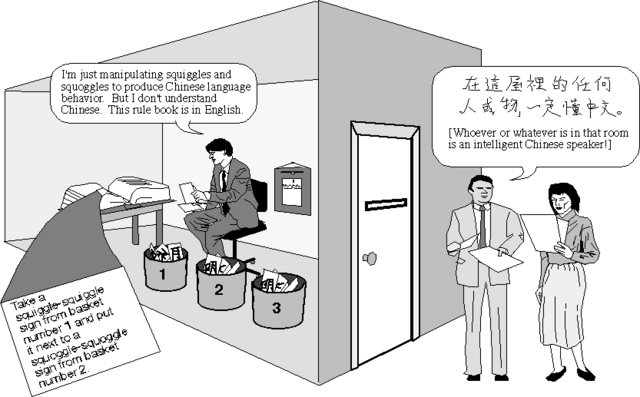
\includegraphics[width=.75\textwidth]{chinese-room.png}}  
  \begin{itemize}
  \item symbol grounding (hard to learn from data)
  \item very inflexible (inconsistencies, mathematical proofs)
  \end{itemize}
\end{frame}

\begin{frame}
  \frametitle{Connectionist systems}
  \begin{itemize}
  \item parallel distributed processing units, neural networks
  \item biologically inspired
  \item non-symbolic, sub-symbolic
    \begin{itemize}
    \item learn from data
    \end{itemize}
  \item challenges:
    \begin{itemize}
    \item interpretability
    \item compositionality
    \end{itemize}
  \item Research question: how much of intelligent behavior is
    symbolic?
  \item Research question: can we combine symbolic and connectionist
    systems to overcome their individual limitations?
  \end{itemize}
\end{frame}

\begin{frame}
  \frametitle{Motivation}
  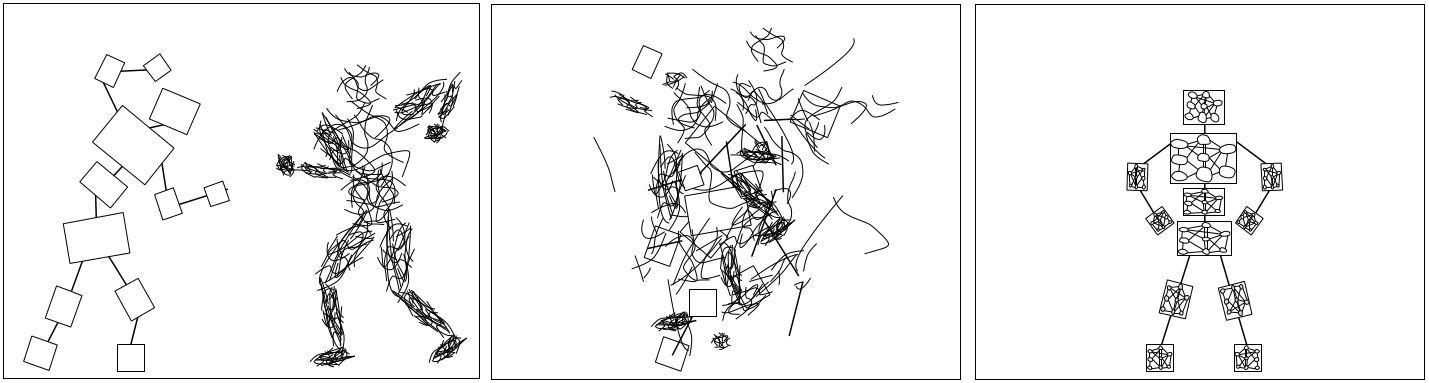
\includegraphics[width=\textwidth]{minsky-figure.png}
\end{frame}

% Limitations of Learning and Reasoning Systems
\begin{frame}
\frametitle{Limitations of Learning and Reasoning Systems}
\begin{itemize}
\item Learning Systems: Data hungry, limited transfer, brittle,
  opaque, no use of prior knowledge
\item Symbolic Reasoning Systems: Brittle, limited scope,
  combinatorial explosions
  \pause
\item The limitations of each approach are largely {\em
    complementary}!
\end{itemize}
\end{frame}

% Complementarity of Techniques
\begin{frame}
\frametitle{Complementarity of Techniques}
\begin{itemize}
\item Statistical learning successful in pattern recognition
\item Symbolic reasoning effective in planning and diagnosis
\end{itemize}
\end{frame}

% Task-Based Distinction
\begin{frame}
\frametitle{Task-Based Distinction}
\begin{itemize}
\item Deduction vs. Induction vs Abduction:
  \begin{itemize}
  \item Classical distinction between reasoning and learning and diagnosis/explanation
  \end{itemize}
\item Compression vs. Decompression:
  \begin{itemize}
  \item Learning as compression
  \item reasoning as decompression
  \end{itemize}
\end{itemize}
\end{frame}

\begin{frame}
  \frametitle{Deduction vs induction}
  \begin{itemize}
  \item Deduction: Given a set of formulas $T$ and a specific
    deductive calculus $\vdash$, derive the specific conclusion
    $\phi$
  \item Induction: Given a set of specific observations
    $\phi_1,...,\phi_n$, find $T$ such that $T \vdash \phi_i$ for all
    $1 \leq i \leq n$
  \item Abduction: Given a set of statements $T$, a specific
    observation $\phi$, and a specific deductive calculus $\vdash$,
    find a statement $\psi$ such that
    $T \cup \{ \psi \} \vdash \phi$
  \end{itemize}
\end{frame}

\begin{frame}
  \frametitle{Compression and decompression}
  \begin{itemize}
  \item Learning as compression: ``compress'' observations
    $\phi_1,...,\phi_n$ into a smaller model $T$
    \begin{itemize}
    \item using any kind of regularity in the data to compress
    \end{itemize}
  \item Reasoning as decompression: produce ``prediction'' $\phi$ from
    model $T$
    \begin{itemize}
    \item $\phi$ was already implicit in $T$
    \item reasoning/deduction to make it explicit
    \end{itemize}
  \end{itemize}
\end{frame}

% Representation-Based Distinction
\begin{frame}
\frametitle{Representation-Based Distinction}
\begin{itemize}
\item ``Model-Free'' Representations: Predominant in learning systems
\item ``Model-Based'' Representations: Typical in reasoning systems.
\item Properties: Compositional, referential, homologous,
  interpretable, symbolic, discrete
\end{itemize}
\end{frame}

\begin{frame}
  \frametitle{Taxonomy of neuro-symbolic systems (Kautz, AAAI 2020)}
  \begin{itemize}
  \item symbolic Neuro symbolic
  \item Symbolic[Neuro]
  \item Neuro;Symbolic
  \item Neuro:Symbolic $\rightarrow$ Neuro
  \item Neuro$_{symbolic}$
  \item Neuro[Symbolic]
  \end{itemize}
\end{frame}

\begin{frame}
  \frametitle{symbolic Neuro symbolic}
  \centering
  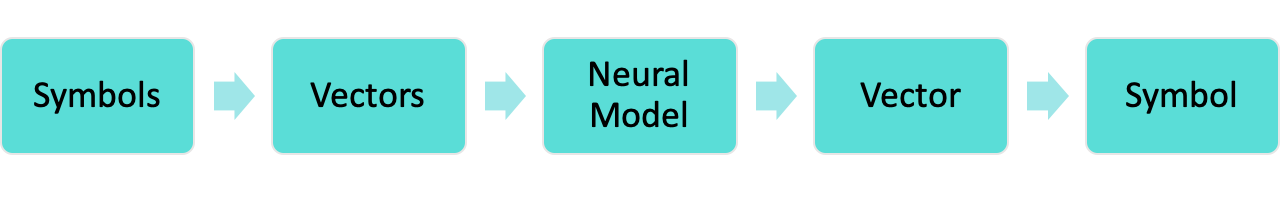
\includegraphics[width=.7\textwidth]{ns10.png}
  \begin{itemize}
  \item symbols as input and output
  \end{itemize}
  % basic pattern above; most NLP is this type
\end{frame}

\begin{frame}
  \frametitle{Symbolic[Neuro]}
  \centering
  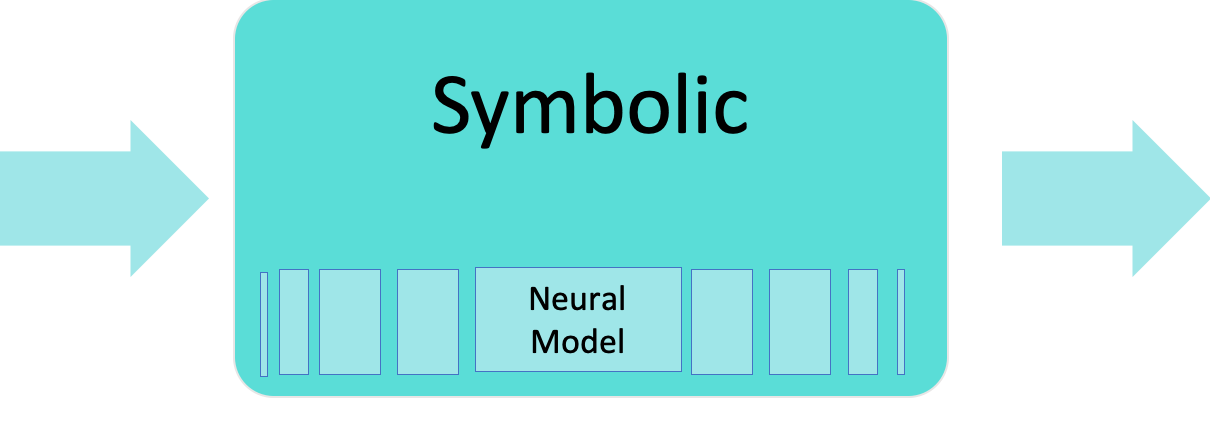
\includegraphics[width=.7\textwidth]{ns11.png}
  \begin{itemize}
  \item symbolic solver, use neural model internally
    % \begin{itemize}
    % \item e.g., search strategy
    % \end{itemize}
  \end{itemize}
  % reinforcement learning for search for proof
  % AlphaGO
\end{frame}

\begin{frame}
  \frametitle{Neuro; Symbolic}
  \centering
  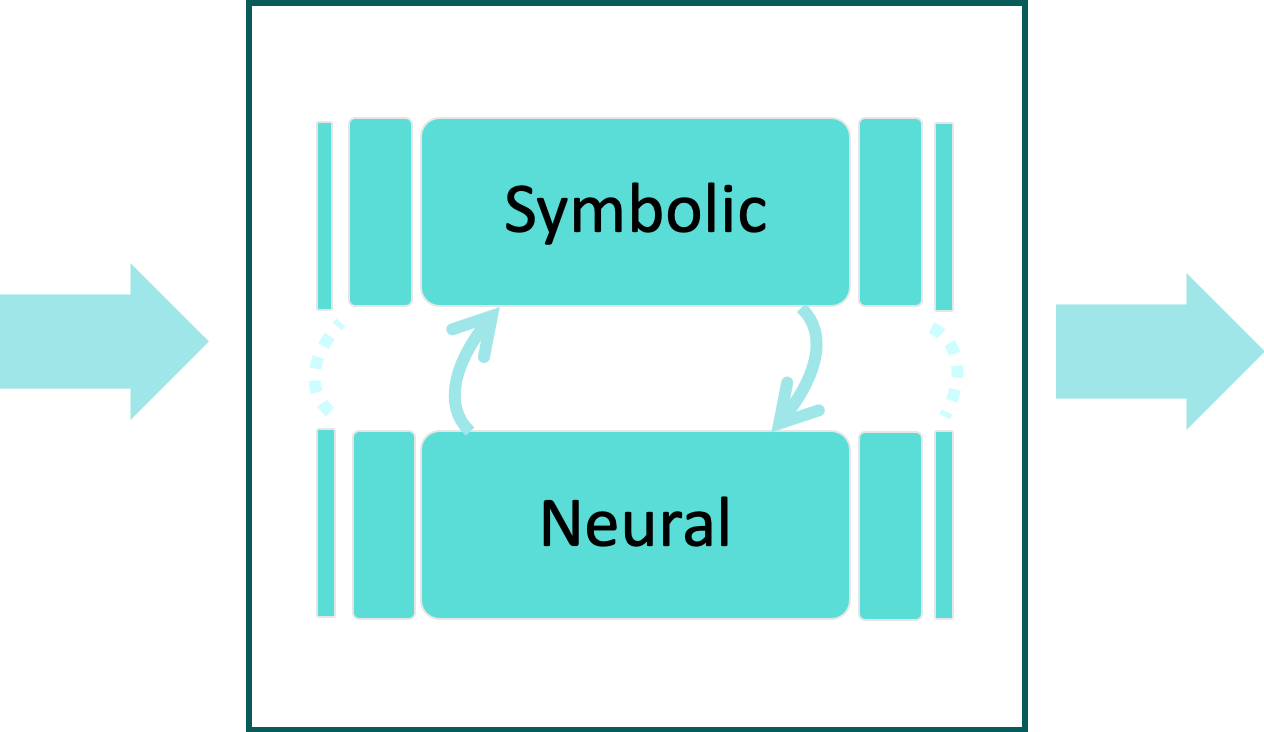
\includegraphics[width=.7\textwidth]{ns12.png}
  \begin{itemize}
  \item symbols from data, then reason
  \end{itemize}
\end{frame}

\begin{frame}
  \frametitle{Neuro:Symbolic $\rightarrow$ Neuro}
  \centering
  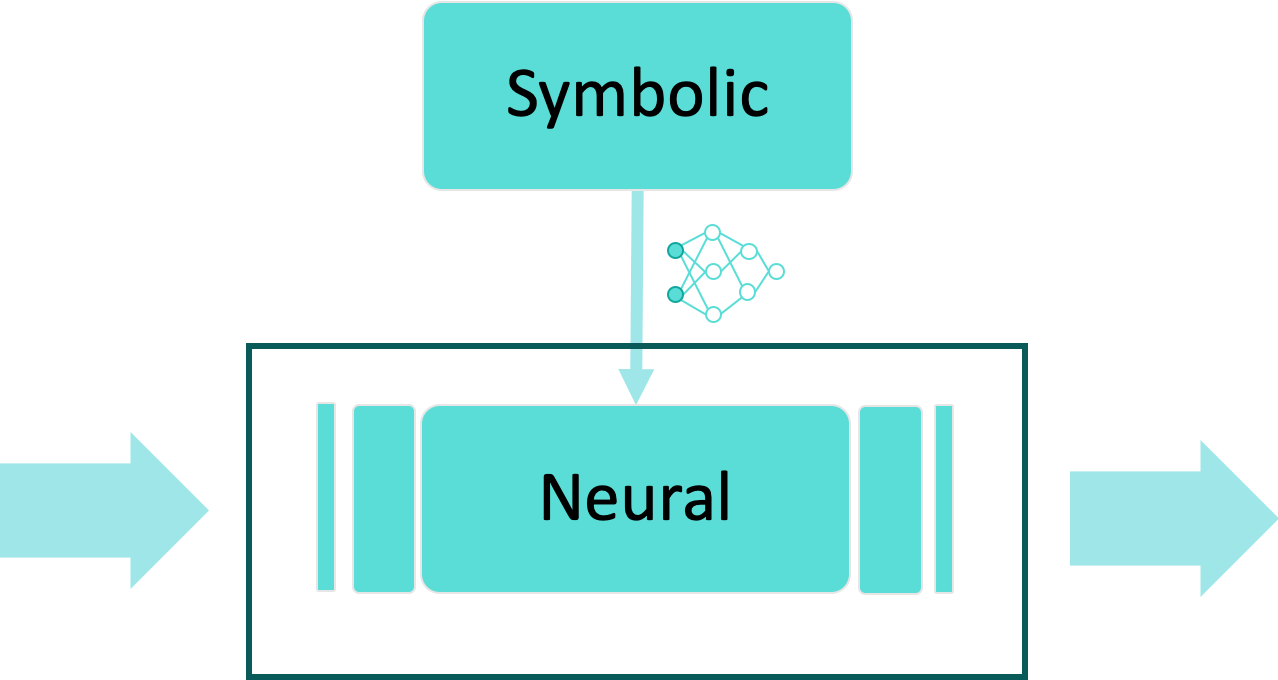
\includegraphics[width=.7\textwidth]{ns13.png}
  \begin{itemize}
  \item symbolic knowledge translated into neural model structure
  \end{itemize}
\end{frame}

\begin{frame}
  \frametitle{Neuro$_{symbolic}$}
  \centering
  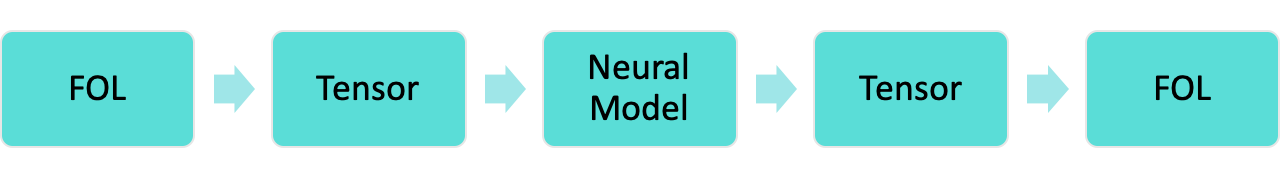
\includegraphics[width=.7\textwidth]{ns14.png}
  \begin{itemize}
  \item symbolic manipulation as neural operations
    % Pattern 7, learning with prior knowledge
  \end{itemize}
\end{frame}

\begin{frame}
  \frametitle{Neuro[Symbolic]}
  \centering
  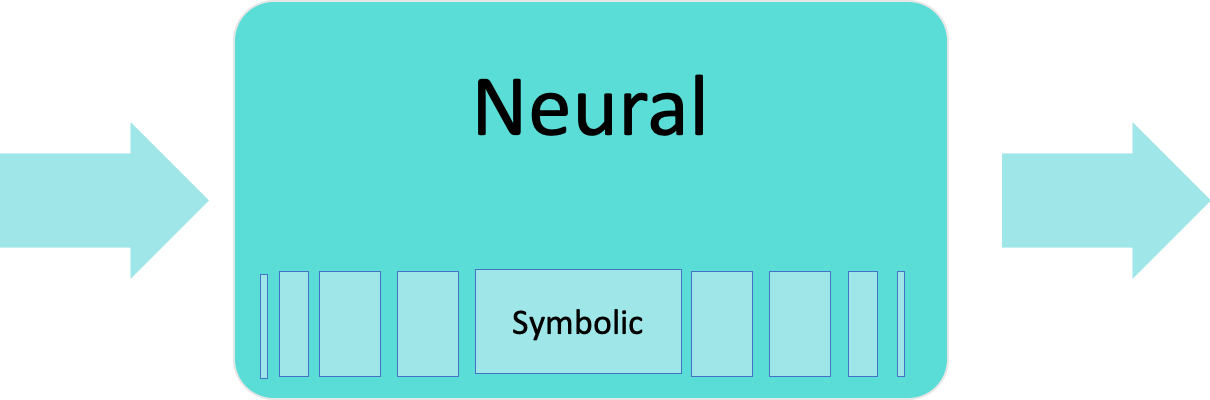
\includegraphics[width=.7\textwidth]{ns15.png}
  \begin{itemize}
  \item learning relation between symbols
  \item attention on particular symbols
    % This is basically what GNNs do (?)
  \end{itemize}
\end{frame}

% Design Patterns and Notation
\begin{frame}
\frametitle{Design Patterns and Notation}
\begin{itemize}
\item Design patterns: General reusable solutions, e.g., in software
  design
\item Hierarchical taxonomy and graphical notation
\item Examples: Software Engineering (Design Patterns), Knowledge
  Engineering (CommonKADS), Ontology Engineering
\item Here: a ``boxology'' introduced by Frank van Harmelen and
  Annette ten Teije
  \begin{itemize}
  \item boxes and arrows
  \item no semantics
  \end{itemize}
\end{itemize}
\end{frame}

\begin{frame}
  \frametitle{Design Patterns and Notation}
  \begin{itemize}
  \item oval nodes: algorithmic components
    \begin{itemize}
    \item deduction: \Ovalbox{KR}
    \item learning: \Ovalbox{ML}
    \end{itemize}
  \item rectangular nodes: inputs, outputs
    \begin{itemize}
    \item model-based, symbolic, relational structures: \fbox{sym}
    \item model-free: \fbox{data}
    \end{itemize}
  \item maybe special node for ``model''
  \end{itemize}
\end{frame}

\begin{frame}
  \frametitle{Design Patterns and Notation}
  \begin{itemize}
  \item \fbox{sym} boxes are inputs and outputs of (traditional) KR
    reasoning systems:
    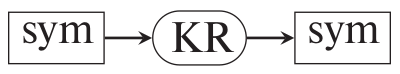
\includegraphics[width=.25\textwidth]{ns1.png}
  \item \fbox{data} boxes are inputs and outputs of (traditional)
    machine learning systems:
    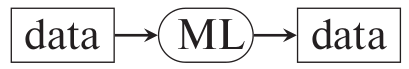
\includegraphics[width=.25\textwidth]{ns2.png}
  \end{itemize}
\end{frame}

\begin{frame}
  \frametitle{Generating models}
  \centering
  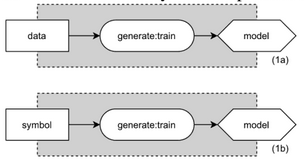
\includegraphics[width=.5\textwidth]{ns3.png}
\end{frame}

\begin{frame}
  \frametitle{Inference}
  \centering
  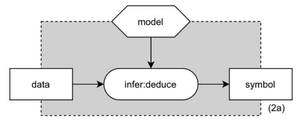
\includegraphics[width=.5\textwidth]{ns4.png}
  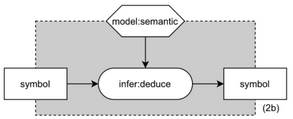
\includegraphics[width=.5\textwidth]{ns5.png}
\end{frame}

\begin{frame}
  \frametitle{Machine learning workflow}
  \centering
  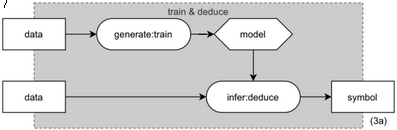
\includegraphics[width=.7\textwidth]{ns6.png}
\end{frame}


\begin{frame}
  \frametitle{Hybrid systems}
  \centering
  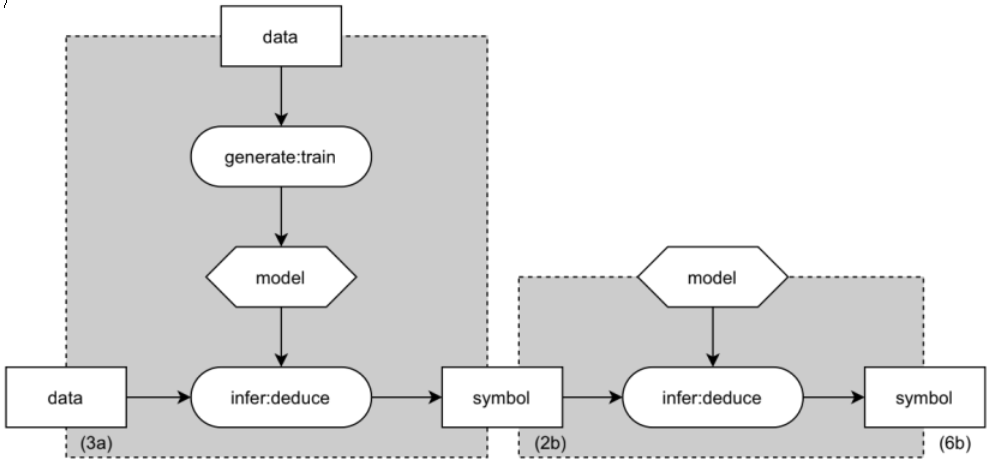
\includegraphics[width=.7\textwidth]{ns7.png}
  % AlphaGO
\end{frame}

\begin{frame}
  \frametitle{Learning an intermediate representation}
  \centering
  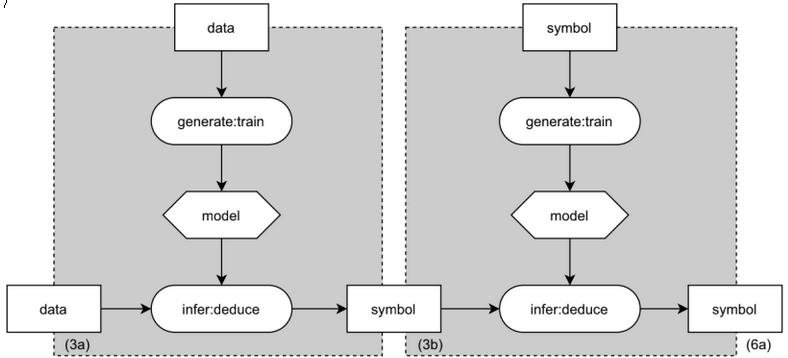
\includegraphics[width=.7\textwidth]{ns8.png}
  % DeepProbLog
  % DeepMind's Atari experiment
\end{frame}

\begin{frame}
  \frametitle{Learning with prior knowledge}
  \centering
  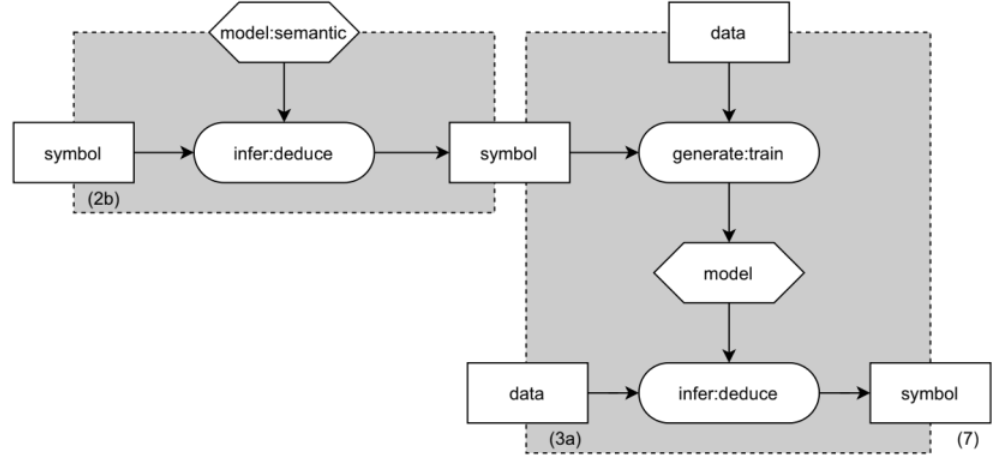
\includegraphics[width=.7\textwidth]{ns9.png}
  % knowledge graphs/bases as symbolic prior
  % semantic loss function (degree to which symbolic knowledge is
  % violated)
\end{frame}

\begin{frame}
  \frametitle{Explanation}
  \centering
  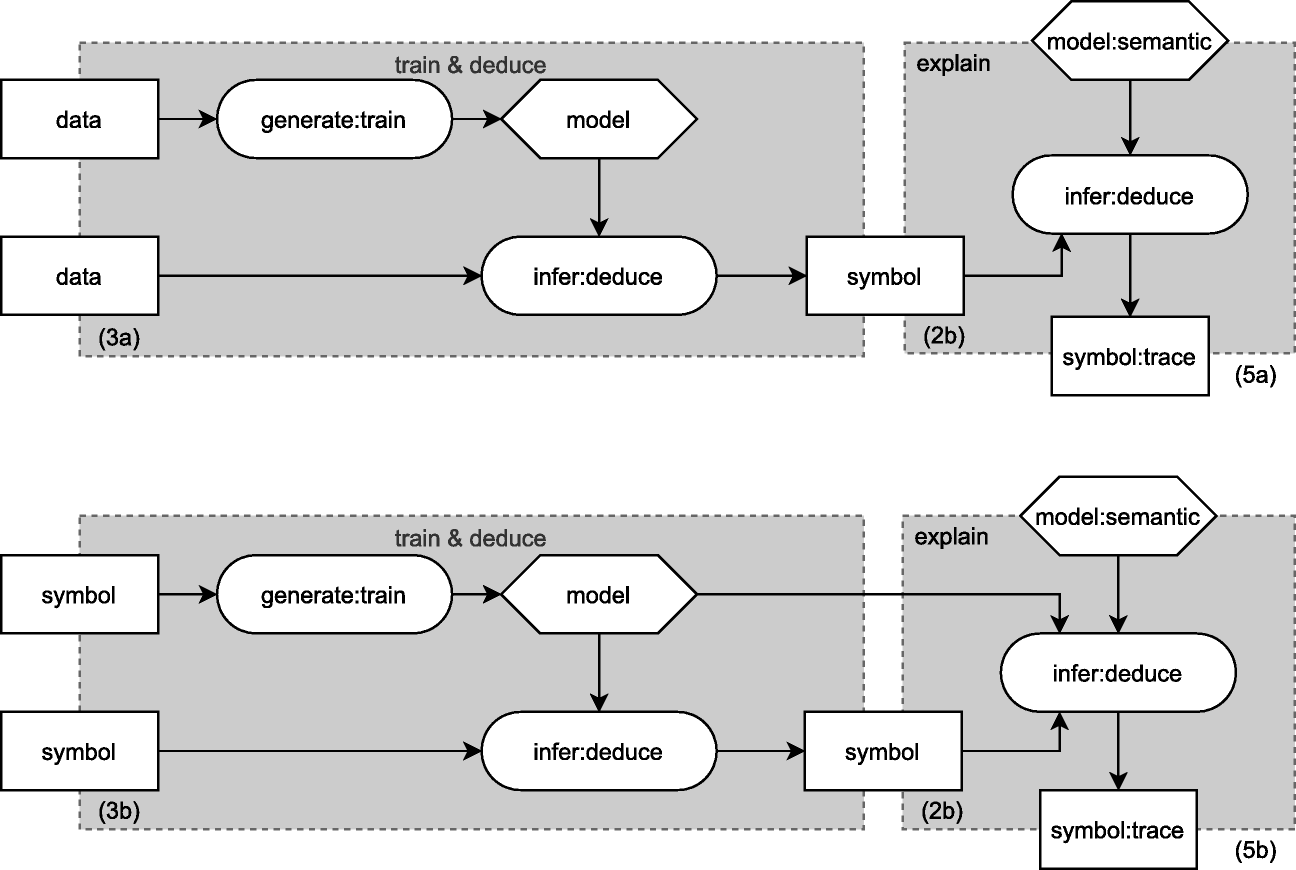
\includegraphics[width=.7\textwidth]{im1.png}
\end{frame}

\begin{frame}
  \frametitle{Learning to reason}
  \centering
  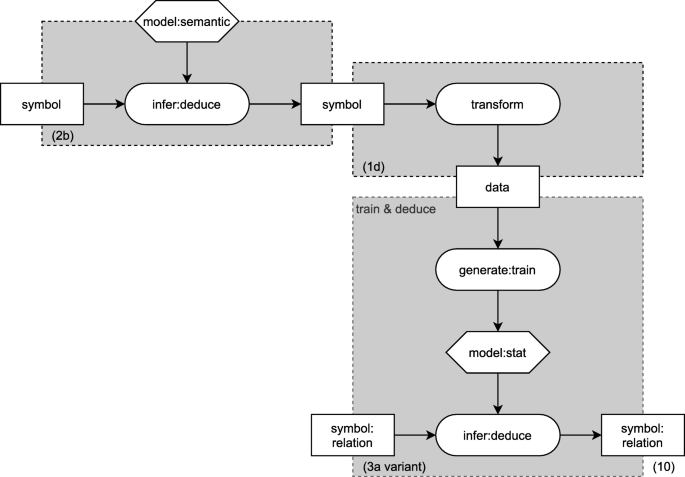
\includegraphics[width=.7\textwidth]{im2.png}
\end{frame}

\begin{frame}
  \frametitle{Other dimensions (Raedt et al., 2020)}
  \begin{itemize}
  \item directed vs un-directed models
  \item model-theoretic vs. proof-theoretic inference
  \item Logic vs. Neural
  \item Boolean vs. probabilistic semantics
  \item Structure vs. parameter learning
  \item Symbols vs. Sub-symbols
  \item Type of Logic
  \end{itemize}
\end{frame}

\begin{frame}
  \frametitle{Other dimensions}
  \centering
  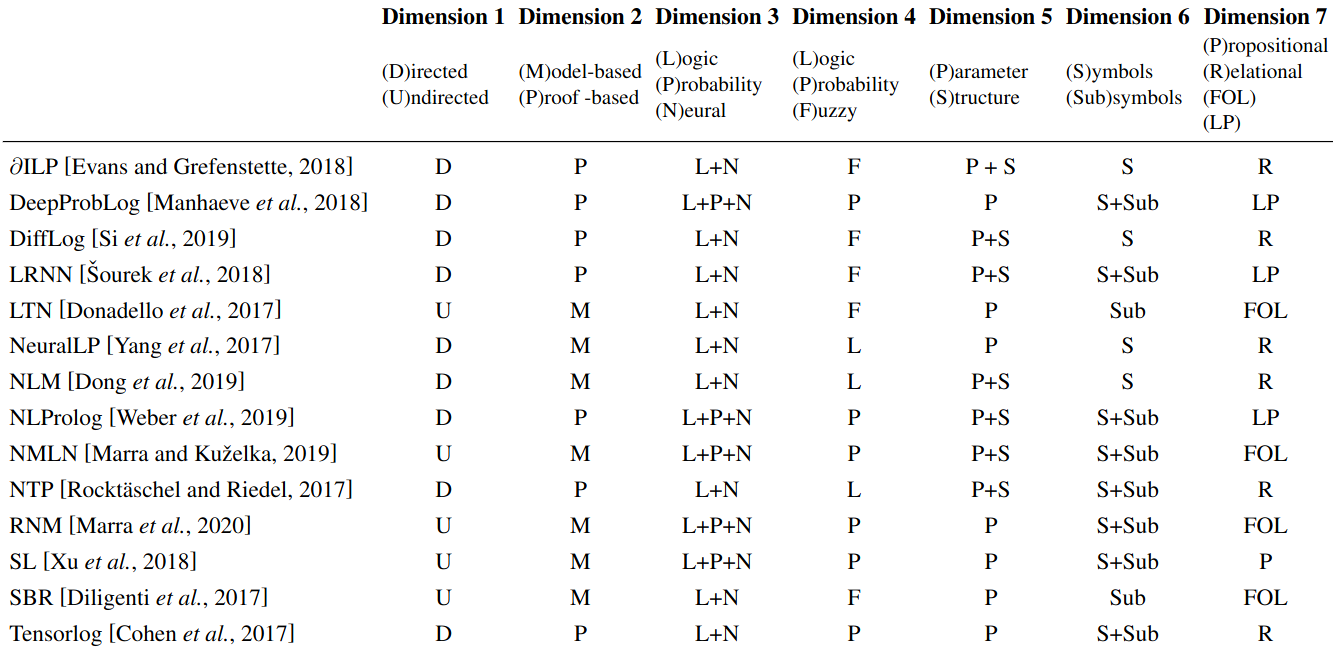
\includegraphics[width=1\textwidth]{im3.png}
\end{frame}

\begin{frame}
  \frametitle{Applications of Neuro-Symbolic methods}
  \begin{itemize}
  \item Solve much harder problems
    \begin{itemize}
    \item few shot, zero shot
    \item deduction
    \end{itemize}
  \item Learn with dramatically less data, ultimately for a large
    number of tasks rather than one narrow task
  \item Provide inherently understandable and controllable decisions
    and actions
  \end{itemize}
\end{frame}

\end{document}

% Introduction:

% Minsky's paper

% http://arxiv.org/abs/1905.12389

% http://arxiv.org/abs/2305.08876

% http://arxiv.org/abs/2302.02093




% From knowledge graph to knowledge base completion


% Neural logical query answering

%%% Local Variables:
%%% mode: latex
%%% coding: utf-8
%%% TeX-master: t
%%% eval: (TeX-run-style-hooks "beamer")
%%% End:
